\documentclass{article}
\usepackage{amsmath,tikz,algorithm2e}
\usetikzlibrary{matrix,calc}
\title{Computer\/ Robot Vision: Lecture 4}
\author{Sam Barrett}

\begin{document}
\maketitle

\section{Image Texture}
\label{sec:texture}

Texture is a very important factor in understanding properties of an object however they can be difficult to define due to potential near random patterns.

We can use texture to:

\begin{itemize}
  \item estimate surface orientation or shape.
  \item classify/ segment an image. Allowing us to group image regions with consistent texture.
        \item synthesise new texture patches or entire images given some example set.
\end{itemize}

By analysing texture we can often identify properties of the material it is made from. Texture acts as a \textit{feature} that is one step abstracted from the basics of filters and edges.

We can think of textures as \textbf{repeated local patterns}. This reduces the first stage of our task of analysing texture to finding patterns. Patterns can include: spots, bars, raw patches etc. We describe textures with statistics related to their local window including mean, standard deviation etc.

We can use our $x$ and $y$ derivative filters to find the texture \textit{responses} in each section of an image. We can then find local statistics by moving a arbitrarily large \textit{window} across the image.

Having calculated this information we can identify all windows in the image with high vertical or horizontal (or both) activity, these areas are likely to have \textit{texture} following these directions. Colour-coding these 4 sets (no intensity, high $x$, high $y$, high $x,y$) we can roughly visualise textures present in the image.

On a plot of mean $\frac{\delta}{\delta x}$ against mean $\frac{\delta}{\delta y}$ the further apart 2 windows are, the more dissimilar their textures. We measure the distance between two points on this plot simply as Euclidean distance ($D(a,b) = \sqrt{\sum_{i=1}^2 (a_{i} - b_{i})^{2}}$)

When performing this form of analysis, the window size we use is very important. If our window is close ins size to an object of interest, made up of multiple textures, we will lose a lot of information.

So far, we have discussed using 1st order derivative filters to find texture information. We can more generally say that we aapply a collection of multiple, $d$, filters called a \textit{filter bank}. This results in feature vectors in $d$ dimensions. We can still consider \textit{nearness} as the Euclidean distance but now we consider it in $d$ dimensional space. This is a simple extension to the previous equation:

\[
  D(a,b) = \sqrt{\sum_{i=1}^d (a_{i} - b_{i})^2}
\]



\subsection{Filter Banks}

We design filter banks so that they cover most bases of possible textures. They contain filters specific to edges, bars, spots or any other textural feature that we are interested in.

Many of these different filters are \textbf{multivariate Gaussian} filters. Multivariate Gaussian filters can be stretched and contorted to respond to different shapes through \textbf{manual} tuning of its parameters. Multivariate Gaussian filters have the form:

\[
  p(x ; \mu, \Sigma) = \frac{1}{(2\pi)^{n/2}|\Sigma|^{1/2}}\exp\left(-\frac{1}{2}(x-\mu)^{T}\Sigma^{-1}(x-\mu)\right)
\]

By changing the parameter $\Sigma$ we can change the direction and distribution of the filter.

More recent work has been done to \textit{learn} filter banks using Convolutional Neural Networks. Here highly specialised filters are learnt from a training set in order to closely match the domain in which the model will be deployed.

CNNs use different levels of filter banks, low level features include basic edges and textures, mid-level filters detect more precise but still abstract features and high-level filters are more concrete still, detecting exact patterns or even objects.

\subsection{Texture Synthesis}

There are many applications for being able create new samples of a given texture:

\begin{itemize}
  \item Virtual environments (games, VR, etc.)
  \item Hole-filling on images
  \item Texturing surfaces
\end{itemize}

The challenge with this sort of task the spectrum of textures we are trying to replicate, ideally with a single general solution. We want to model both repeated and stochastic (random) textures.

\subsubsection{Markvov Chains}

A Markov chain is a sequence of random variables $x_{1}, x_{2}, \ldots, x_{n}$ where $x_{t}$ is the state of the model at a given time $t$.

They have been used for text synthesis, with the most basic implementations building a probability histogram or table featuring the probabilities of a word being present given the previous words seen ($p(x_{t} | t_{t-1},\ldots,x_{t-(n-1)})$)

More modern approaches use machine learning models such Long-short-term-memory networks or LSTMs. The results of these models are better but still often nonsensical.

We can extend the approach of Markov chains to help us to predict and synthesise textures in images. We do this using \textbf{Markov random fields} (MRF), these are generalisations of Markov chains to be in 2 or more dimensions.

A first order MRF (works on 2 dimensions) computes the probability that pixel $X$ takes a certain value \textbf{given} the values of neighbours $A,B,C,D$, $P(X | A,B,C,D)$

\begin{center}
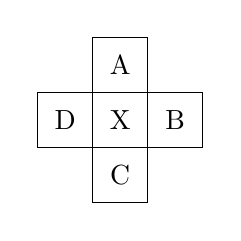
\begin{tikzpicture}
\matrix (m) [matrix of nodes,
             nodes={minimum size=1em, outer sep=0pt,inner sep=0,line
             width=0.5pt,append after command={\pgfextra{\draw
             ($(\tikzlastnode.north west)+(-0.5em,+0.5em)$)
             rectangle ($(\tikzlastnode.south east)+(0.5em,-0.5em)$);}}},
             column sep=-0.5pt, row sep=-0.5pt
              ]
              {
                & A & \\
                D & X & B \\
                & C & \\
  };
\end{tikzpicture}
\end{center}

\subsubsection{Single pixel synthesis}

In order to synthesise a value for a single pixel $x$ we need to calculate $P(x | \text{neighbourhood of pixels around }x)$.

To do this we:

\begin{itemize}
  \item first find all windows \textbf{elsewhere in the image} that match the neighbourhood of $x$.
  \item Pick 1 matching window at random, $W$
  \item assign $x$ the centre pixel of $W$.
\end{itemize}

Often an exact neighbourhood match will not exist, so we find the best matches using sum of squared differences (SSD) error and choose between them with a weighted probability, preferring \textit{better} matches.

The size of our neighbourhood window effects the predictions we make. It must be set according to the texture being synthesised. Brickwork, for example, should not be synthesised using a window bigger than a single brick etc.


\subsubsection{Efros \& Leung algorithm}

This is the algorithm for synthesising texture pixel-by-pixel, it is \textbf{simple}, yields \textbf{good results} but is \textbf{very slow}.

\subsubsection{Efros \& Freeman algorithm}

This is an improved version of the Efros and Leung algorithm, it is based on the observation that neighbourhood pixels are highly correlated. The main idea is to use a \textit{block} as the base unit of synthesis rather than a single pixel.

This changes our conditional probability calculation to $P(\mathbf{B} | N(\mathbf{B} ))$, this is much faster as we now synthesise all pixels in $\mathbf{B} $ at once.

The layout of blocks used greatly effects performance of this algorithm.

\begin{itemize}
  \item Placing blocks randomly that do not overlap results in sharp, unnatural edges in the synthesised texture
  \item Making neighbouring blocks overlap produces better but still unnatural results.
  \item The minimal error boundary cut approach produces the best result

        This approach is done by overlapping 2 blocks. The edge between them is clear so we take the two overlapping sections of each block and calculate the overlap error. This error gives us the \textit{minimal error boundary}, cutting each block along this boundary allows us to accurately stitch these two blocks together.

        This approach can be seen in Figure~\ref{fig:meb}
\end{itemize}

\begin{figure}[ht]
  \centering
  \includegraphics[scale=0.3]{figures/l4-1.png}
  \caption{\label{fig:meb} Minimal error boundary calculation}
\end{figure}

\subsection{Texture Transfer}

Texture transfer is the process of mapping a texture from one object to another. This requires being able to separate texture from the shape of an object.

This is very difficult to do, so we cheat. We assume we can capture shape through boundaries and rough shading, then we just add similarity to underlying image at the same point as a constraint when sampling.

\section{Image Segmentation}

\subsection{Grouping in vision}

The goal of grouping in computer vision is to:

\begin{itemize}
  \item Collect features that belong together

        This can include determining image regions by colour or texture, or grouping video frames into \textit{shots} to help us extact people or objects from a video.

  \item Obtain an intermediate representation that compactly describes key image or video components
\end{itemize}

There are two main approaches to grouping: \textbf{Top-down} and \textbf{bottom-up} segmentation.

Top down segmentation means that pixels belong together as they are from the same object. This approach requires prior knowledge about objects in the image, we then infer that similar pixels are together.

Bottom up segmentation means that pixels belong together as they \textit{look} similar.

\subsection{Bottom up segmentation}

Algorithms include $k$-means clustering and mean-shift clustering. There are also graphical approaches.

The goals of segmentation are to:

\begin{itemize}
  \item separate images into coherent \textit{objects}.
  \item group together similar looking pixels.

        This is for efficiency of later processing. These blocks of similar pixels are known as \textit{super-pixels} and are very useful for higher level processing.

\end{itemize}

\subsubsection{$k$-means clustering}

\begin{algorithm}
  \caption{$k$-means clusering}
  Randomly initialise the cluster centres $c_{1},\ldots,c_{k}$

  \While{cluster assignments change}{
    \ForEach{each point $p$}{find the closest centre $c_{i}$, place $p$ into cluster $i$}
    \ForEach{cluster, $c_{i}$}{
        Calculate new centroid (mean point in cluster)
    }
  }
\end{algorithm}

This algorithm will \textbf{always converge} to some solution. However, this can be a local minimum. I.e. it does nto always find the global minimum of the objective function $\mathcal{F} = \sum_{i=0}^k \sum_{j=0}^n \| p_{j} - c_{i}\|^{2}$.

It is also very fast and simple to compute. However, setting $k$ is task specific (or inefficient to determine), the process is sensitive to the initial cluster centres as well as to outliers.

We also assume that the means of the our points can be computed.

\subsubsection{Segmentation as clustering}

We can group pixels in different ways based on what we select to be our feature space.

Our feature space can be many different things including (but not limited to):

\begin{itemize}
  \item Intensity
  \item Colour similarity (3D feature space)
  \item Intensity and position
  \item Texture similarity
  \item $n$-dimensional feature space
\end{itemize}

\subsubsection{Mean shift algorithm}

The mean shift algorithm looks for \textit{modes} or local maxima of density in the feature space.

\begin{algorithm}
  \caption{Mean shift algorithm}
  Initialise random seed and window $W$

  \While{not converged}{
    calculate the centre of gravity (mean) of $W$

    shift $W$ to the mean
 }
\end{algorithm}

This can be applied to clustering/ segmentation by:

\begin{enumerate}
  \item Finding features based on some feature space (colour, gradients, texture, etc.)
  \item Initialising windows at each individual feature point
  \item Performing mean-shift for each window to convergence
  \item Merge windows that end up near the same \textit{peak} or mode
\end{enumerate}

Advantages of mean-shift

\begin{itemize}
  \item Does not assume shape of clusters ($k$-means assumes spherical clusters)
  \item Single parameter to tune (window size)
  \item Generic technique
  \item Can find multiple modal values
\end{itemize}

Disadvantages of mean-shift:

\begin{itemize}
  \item Manual selection of window size
        \item Does not scale well with dimensionality of feature space (texture etc.)
\end{itemize}

\subsubsection{Graphical approaches}

We can also view images as fully-connected graphs. Each node is a pixel and there is a edge between every pair of pixels.

We can assign an \textit{affinity weight}  to each edge $w_{p,q}$ measures similarity.

One definition for affinity is:

\[
  \textit{aff}(x,y) = \exp\left\{-\left(\frac{1}{2\sigma^{2}_{d}}\right)(\|x-y\|^{2})\right\}
\]

Where small values of \(\sigma\) will group only nearby points and large values of \(\sigma\) will group distant points.

With a image graph and this notion of affinity, we can break graph into segments. We want to remove edges that cross between segments. The easiest method breaks the links that have low similarity. This means that similar pixels should be in the same segments.

\paragraph{MinCut}

We can construct a notion of \textbf{MinCut}, the set of links in a graph $G$ with two subgraphs representing segments $A,B$ whose removal makes $G$ disconnected. The cost of a cut is given as:

\[
  \textit{cut}(A,B) = \sum_{p\in A, q\in B} w_{p,q}
\]

Finding \textbf{MinCut}  gives us a segmentation of the image represented by $G$, there exist efficient algorithms to find this.

The issue with this is that the weight of a cut is proportional to the number of edges in the cut. This means it tends to produce small, isolated components.

\paragraph{Normalised cut}

Normalised cut is a MinCut alternative. Here we fix the bias of \textbf{MinCut} by normalising the size of the segments.

\[
  \textit{Ncut} (A,B) = \frac{\textit{cut} (A,B)}{\textit{assoc}(A,V) } + \frac{\textit{cut}(A,B) }{\textit{assoc}(B,V) }
\]

Where $\textit{assoc}(A,V) $ is the sum of weights of all edges that touch $A$.

The value of \textit{Ncut} is small when we get two clusters with many edges with high weights and few edges of low weight between them. The a solution to $\min(\textit{Ncut} )$  is approximately the same as the generalised eigenvalue problem.

Advantages of normalised cuts

\begin{itemize}
  \item Generic framework, flexible choice of definition for \textit{affinity}, which assigns weight to edges.
        \item Does not require model of data distribution
\end{itemize}

Disadvantages:

\begin{itemize}
  \item Can have high time complexity, dense graphs require many affinity calculations. Also solving the eigenvalue problem is non-trivial
        \item It has a preference for balanced partitions.

\end{itemize}

There is an efficient graph-based segmentation approach, it runs in time linear in the number of edges, it is easy to control coarseness of segmentation however, the results can be unstable.

\section{Fitting}

In fitting we aim to select a parametric model that best represents a set of features.

We know that membership of a model cannot be determined on a point-local basis, we must consider surrounding pixel values also.

We can reduce fitting to three main questions:

\begin{enumerate}
  \item What model represents this set of features best?
  \item Which of several model instances get which feature?
  \item How many model instances are there?
\end{enumerate}

When considering fitting we must be mindful of time complexity, it is not computationally feasible to examine every possible set of parameters and every possible combination of features.

\subsection{Line fitting}

The simplest type of feature we often wish to fit are straight lines. Many objects are characterised by the presence of straight lines.

But why can this not be achieved simply through edge detection?

There are often multiple extra edge points in an image which can lead to clutter in our models as we ask the question \textit{which points go with which lines, if any?}

Sometimes only sections of a line are detected, how do we find lines that span sections of an image with imperfect information?

There is often noise in measured edge points and orientations, how do we remove noise to detect the true underlying parameters?

\subsection{Voting}

We have said that it is not feasible to check all combinations of features by fitting a model to each possible subset. \textbf{Voting} is a general technique whereby we let each feature \textit{vote} for all models that are compatible with it.

It works by cycling through features and casting votes for model parameters, we then look for the model parameters that receive the most votes.

Features created due to noise and clutter will still vote in this system but generally their votes should be outweighed by the larger set of \textit{``good''} features.

\subsection{Hough Transforms}

Hough Transforms are a voting technique used to determine the following information:

\begin{itemize}
  \item Given some point that belong to \textit{a} line, what is the line?
  \item How many lines are there in a given image?
  \item Which points belong to which line?
\end{itemize}

The main idea behind this technique is:

\begin{itemize}
  \item each straight line in an image can be described by a (unique) equation
  \item Each point on this line, when considered in isolation, could lie on an infinite number of other straight lines
  \item In the Hough Transform, each point votes for every line it could be on; the lines with the most votes \textit{win}
\end{itemize}

\paragraph{How do we represent lines?}

Any line can be represented using 2 numbers, $w \text{ and } \phi$. We say a line is a line from an agreed origin of length $w$ at an angle $\phi$ to the horizontal.

Since we can use $(w,\phi)$ to represent any line in the image space, we can represent any line in the image space as a point in the plane defined by $(w,\phi)$, we call this plane the \textbf{Hough Space}.

\paragraph{How does a point in the image space vote?}

We can transform a point in the image space to a sinusoidal curve in the Hough Space through the equation:
\[
  w = x \cos(\phi) + y \sin(\phi)
\]

Therefore, two points in the image space correspond to two curves in the Hough space. The intersection of those two curves has two \textit{votes} . This intersection represents the straight line in the image space that passes through both points.

The basic Hough Transform algorithm is:

\begin{algorithm}
  \caption{Hough Transform}
  Create an array $\texttt{A} $ indexed by $\phi$ and $w$

  \ForEach{point $(x,y)$ in the image space}{
    \ForEach{angle $\phi \in [\phi_{\text{min}},\phi_{\text{max}}]$}{
      $w = x\cos(\phi) + y\sin(\phi)$

      $\texttt{A}[\phi,w] = \texttt{A}[\phi,w]+1  $
    }
  }

  Find the value(s) of $w,\phi$ where $\texttt{A}[w,\phi] $ is maximum

  The detected line in the image is given by $w = x\cos(\phi) + y\sin(\phi)$
\end{algorithm}

When we have a noisy image however, we still see votes being cast in the Hough space. This can lead to false positives.

We can extend Hough transform to include the gradient direction, this is a piece of information that we calculate during the edge detection phase.

We can alter our algorithm to form:

\begin{algorithm}
  \caption{Hough Transform}
  Create an array $\texttt{A} $ indexed by $\phi$ and $w$

  \ForEach{point $(x,y)$ in the image space}{
    $\phi = $ gradient at $(x,y)$

      $w = x\cos(\phi) + y\sin(\phi)$

      $\texttt{A}[\phi,w] = \texttt{A}[\phi,w]+1  $
  }

  Find the value(s) of $w,\phi$ where $\texttt{A}[w,\phi] $ is maximum

  The detected line in the image is given by $w = x\cos(\phi) + y\sin(\phi)$
\end{algorithm}

This reduces the degrees of freedom.

Other extensions that we can make are:

\begin{itemize}
  \item Give more votes to stronger edges by incorporating the magnitude of the gradient
  \item Change the sampling of $w, \phi$ to increase or reduce the resolution
  \item We can extend this procedure for use on circle, square or any other regular shape.
\end{itemize}

\subsubsection{Hough Transform for circles}

Given a circle of centre $(a,b)$ and radius $r$ we define it parametrically as:

\[
  (x_{i} - a )^{2} + (y_{i} - b)^{2} = r^{2}
\]
\paragraph{Known $r$}
For a known radius $r$ the parameter space is reduced to 2D, each point represents the centre of a circle. For each point $(x,y)$ on the original circle, there is a corresponding circle centred at $(x,y)$ with a radius $r$ in the Hough space. The intersection point of all such circles in the Hough space would be corresponding to the centre point of the original circle. See Figure~\ref{fig:cht}

\begin{figure}[ht]
  \centering
  \includegraphics[scale=0.3]{figures/l4-2.jpg}
  \caption{\label{fig:cht} Circle Hough Transform}
\end{figure}

\paragraph{Unknown $r$}
In the case where the radius, as well as the centre, is unknown, the parameter space (Hough space) is 3 dimensional. Each point in the image space corresponds to a cone in the Hough space. The point of the cone is at $r=0,x,y$. We can still find the set of parameters that gain the most votes in the Hough space by finding intersections between these cones. See Figure~\ref{fig:unknown-r-ht}

\begin{figure}[ht]
  \centering
  \includegraphics[scale=0.3]{figures/l4-3.png}
  \caption{\label{fig:unknown-r-ht} Circle Hough Transform for an unknown $r$ }
\end{figure}

\paragraph{Unknown radius, known gradient direction}

This is a subset of the previous case. By knowing the gradient direction, we make our calculation much simpler. Every point in our image space now becomes a single straight line in the Hough space. Votes are cast by finding intersections between these lines. See Figure~\ref{fig:known-gd-ht}

\begin{figure}[ht]
  \centering
  \includegraphics[scale=0.3]{figures/l4-4.png}
  \caption{\label{fig:known-gd-ht} Known gradient direction Hough Transform}
\end{figure}

In this case, we can re-arrange our circle equation into the form:

\begin{align*}
  x &= a + r\cos \theta \\
  y &= b + r\sin \theta
\end{align*}

Here, every point $(x,y)$ in the image space will be equivalent to a circle in the $(a,b)$ Hough space. By rearranging these equations we get:

\begin{align*}
  a &= x_{i} - r\cos \theta\\
  b &= y_{i} - r\sin \theta
\end{align*}

If the radius is know then the centre of the circle can be calculated.

\textbf{UNFINISHED}


\end{document}
